%------------------------------------------------------------------------------
% Author(s):
% Varaun Ramgoolie
% Copyright:
%  Copyright (C) 2020 Brad Bachu, Arjun Mohammed, Nicholas Sammy, Kerry Singh
%
%  This file is part of Applied-Mathematics-Unit2 and is distributed under the
%  terms of the MIT License. See the LICENSE file for details.
%
%  Description:
%     Year: 2010
%     Module: 1
%     Question: 1 
%------------------------------------------------------------------------------
\usetikzlibrary{patterns}

\begin{subquestions}
	
%------------------------------------------------------------------------------
% 1 a--------------------------------------------------------------------------
%------------------------------------------------------------------------------

\subquestion

To maximize, $P = x+2y$, we are given the following inequalities:

\begin{align}
	3x + 17y & \leq 170 \,, \nn \\
	7x + 8y & \leq 175 \,, \nn \\
	y & \leq 9 \,, \nn \\
	x & \leq 2 \,.
\end{align}

\begin{subsubquestions}
	
%------------------------------------------------------------------------------
% 1 a i--------------------------------------------------------------------------
%------------------------------------------------------------------------------

\subsubquestion

The feasible region is shaded in the graph below.


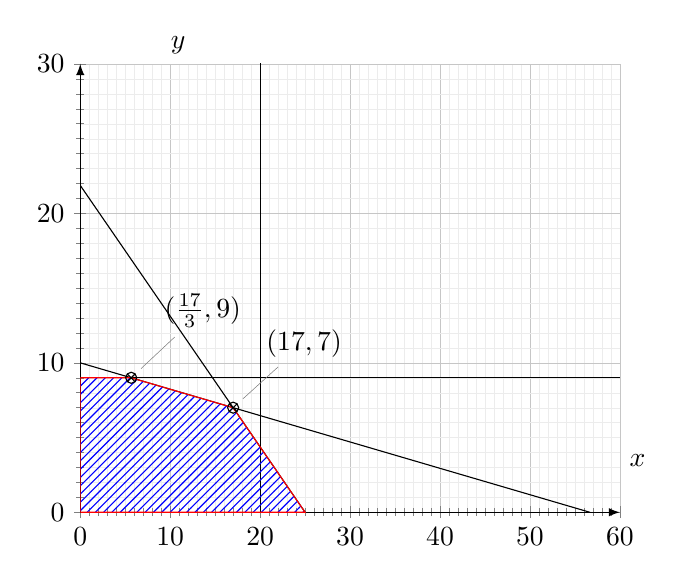
\begin{tikzpicture}
	\begin{axis}
			[
			xmin=-0,xmax=60,
			ymin=0,ymax=30,
			grid=both,
			grid style={line width=.1pt, draw=darkgray!10},
			major grid style={line width=.2pt,draw=darkgray!30},
			axis lines=left,
			minor tick num=9,
			enlargelimits={abs=0},
			axis line style={-latex},
			samples=100,
			domain = -20:20,
			ytick={0,10,...,30},
			xtick={0,10,...,60},
			xlabel={$x$},
			ylabel={$y$},
			x label style={at={(axis description cs:1,0.15)},anchor=north west},
			y label style={at={(axis description cs:0.15,1)},anchor=south west, rotate=-90}
			]
			
			\addplot [mark=dot] coordinates{(170/3, 0)  (0,10)};
			
			\addplot [mark=dot] coordinates {(25,0) (0, 175/8)};
			
			\addplot [mark=dot] coordinates {(0,9) (100,9)};
			
			\addplot [mark=dot] coordinates {(20,0) (20,100)};
			
			\addplot [red,pattern=north east lines,pattern color=blue] coordinates {(0,9) (17/3, 9) (17, 7) (25,0)} \closedcycle;	
			
			\node [pin=60:{$(\frac{17}{3}, 9)$}] at (axis cs:17/3, 9) {};
			
			\addplot [mark=otimes] coordinates{(17/3, 9)};
			
			\node [pin=60:{$(17,7)$}] at (axis cs:17,7) {};
			
			\addplot [mark=otimes] coordinates{(17,7)};
			
	\end{axis}	
\end{tikzpicture}


%------------------------------------------------------------------------------
% 1 a ii-----------------------------------------------------------------------
%------------------------------------------------------------------------------

\subsubquestion

From ~\ref{mod1:defn:TourOfVertices}, we can calculate $P$ by,

\begin{align}
	\text{Using (0,9)} \,, \nn \\
	P & = x + 2y \,, \nn \\
      & = (1 \times 0) + (2 \times 9) \,, \nn \\
	  & = 18 \,. \\
	\text{Using ($\frac{17}{3}$, 9)} \,, \nn \\
	P & = x + 2y \,, \nn \\
	  & = (1 \times \frac{17}{3}) + (2 \times 9) \,, \nn \\
	  & = \frac{71}{3} \approx 23.67 \,.    \\		  
	\text{Using (17,7)} \,, \nn \\
	P & = x + 2y \,, \nn \\
	  & = (1 \times 17) + (2 \times 7) \,, \nn \\
	  & = 31 \,. \label{2010:q1:eqn:Profit} \\
	\text{Using (25,0)} \,, \nn \\
	P & = x + 2y \,, \nn \\
	  & = (1 \times 25) + (2 \times 0) \,, \nn \\
	  & = 25 \,. 
\end{align}

Thus, from \req{2010:q1:eqn:Profit}, the maximum value of $P$ is $31$.

\end{subsubquestions}

%------------------------------------------------------------------------------
% 1 b--------------------------------------------------------------------------
%------------------------------------------------------------------------------

\subquestion

\begin{subsubquestions}
	
%------------------------------------------------------------------------------
% 1 b i--------------------------------------------------------------------------
%------------------------------------------------------------------------------

\subsubquestion

The Hungarian algorithm is shown in \rtab{2010:q1:tab:HungAlgo}.

\begin{table}[!hbt]
	\begin{minipage}{0.3\textwidth}
		\centering
		\begin{tabular}{ccccc}
			50 & 52 & 51 & 54 & 53 \\
		    55 & 53 & 50 & 50 & 52 \\
			49 & 51 & 48 & 53 & 50 \\
			50 & 50 & 52 & 50 & 51 \\
			52 & 54 & 49 & 52 & 24 \\
		\end{tabular}
		\captionsetup{width=1.1\linewidth}
		\caption*{Matrix From question}
	\end{minipage}
%-------------------------------------------------------------------------------
	\hspace{20pt}
	\begin{minipage}{0.3\textwidth}
		\centering
		\begin{tabular}{ccccc}
			0 & 2 & 1 & 4 & 3 \\
			5 & 3 & 0 & 0 & 2 \\
			1 & 3 & 0 & 5 & 2 \\
			0 & 0 & 2 & 0 & 1 \\
			3 & 5 & 0 & 3 & 5 \\
		\end{tabular}
		\captionsetup{width=1.1\linewidth}
		\caption*{Matrix after Reducing Rows}
	\end{minipage}
%-------------------------------------------------------------------------------
	\hspace{20pt}
	\begin{minipage}{0.3\textwidth}
		\centering
		\begin{tabular}{ccccc}
			0 & 2 & 1 & 4 & 2 \\
			5 & 3 & 0 & 0 & 1 \\
			1 & 3 & 0 & 5 & 1 \\
			0 & 0 & 2 & 0 & 0 \\
			3 & 5 & 0 & 3 & 4 \\
		\end{tabular}
		\captionsetup{width=1.1\linewidth}
		\caption*{Matrix after Reducing Columns} 
	\end{minipage}
%-------------------------------------------------------------------------------
	\vspace{20pt} 
	\begin{minipage}{0.3\textwidth}
		\centering
		\begin{tabular} {ccccccc}
   			&   &   & \hspace{-3.25mm} \hvs{v1}        &   &   &  			    \\
   \hhs{h1} & 0 & 2 & 1               				   & 4 & 2 &  \hhe[blue]{h1}\\
   \hhs{h2} & 5 & 3 & 0                                & 0 & 1 &  \hhe[blue]{h2}\\
			& 1 & 3 & 0                                & 5 & 1 &                \\
   \hhs{h3}	& 0 & 0 & 2                                & 0 & 0 &  \hhe[blue]{h3}\\
			& 3 & 5 & 0                                & 3 & 4 &                \\
			&   &   & \hspace{-3.25mm} \hve[blue]{v1}  &   &   &                \\
		\end{tabular}
		\captionsetup{width=1.1\linewidth}
		\caption*{Shading 0's using the least \\ \centering number of lines}
	\end{minipage}
%-------------------------------------------------------------------------------
	\hspace{20pt}
	\begin{minipage}{0.3\textwidth}
		\centering
		\begin{tabular}{ccccc}
			  &   &   &   &   \\
			0 & 2 & 3 & 4 & 2 \\
			5 & 3 & 2 & 0 & 1 \\
			0 & 2 & 0 & 4 & 0 \\
			0 & 0 & 4 & 0 & 0 \\
			2 & 4 & 0 & 2 & 3 \\
			  &   &   &   &   \\
		\end{tabular}
		\captionsetup{width=1.1\linewidth}
		\caption*{Applying Step ~\ref{mod1:defn:HungAlgStep4} \\ \hspace{0pt}} % The reference here is a placeholder until that note is put in%
	\end{minipage}
%-------------------------------------------------------------------------------
	\hspace{20pt}
	\begin{minipage}{0.3\textwidth}
		\centering
		\begin{tabular}{ccccccc}
				&     &   &   &   &    &			   \\
	\hhs{h1}	&	0 & 2 & 3 & 4 & 2  & \hhe[red]{h1} \\
	\hhs{h2}	&	5 & 3 & 2 & 0 & 1  & \hhe[red]{h2} \\
	\hhs{h3}	&	0 & 2 & 0 & 4 & 0  & \hhe[red]{h3} \\
	\hhs{h4}	&	0 & 0 & 4 & 0 & 0  & \hhe[red]{h4} \\
	\hhs{h5}	&	2 & 4 & 0 & 2 & 3  & \hhe[red]{h5} \\
				&	  &   &   &   &    & 			   \\
		\end{tabular}
		\captionsetup{width=1.1\linewidth}
		\caption*{Shading 0's using the least \\ \centering number of lines}
	\end{minipage}

	\caption{\label{2010:q1:tab:HungAlgo} Showing the steps of the Hungarian Algorithm.}
\end{table}

From \rtab{2010:q1:tab:HungAlgo}, the possible pairings for the tasks and persons are,

\begin{align}
	& \text{Person A} \rightarrow 1 \,, \nn \\
	& \text{Person B} \rightarrow 4 \,, \nn \\
	& \text{Person C} \rightarrow 1 ~\text{or} ~3 ~\text{or} ~5 ,, \nn \\
	& \text{Person D} \rightarrow 1 ~\text{or} ~2 ~\text{or} ~4 ~\text{or} ~5 \,, \nn \\
	& \text{Person E} \rightarrow 3 \,.
\end{align}
	
Therefore, the optimum pairings are as follows:

\begin{align}
	& \text{Person A} \rightarrow 1 \,, \nn \\
	& \text{Person B} \rightarrow 4 \,, \nn \\
	& \text{Person C} \rightarrow 5 \,, \nn \\
	& \text{Person D} \rightarrow 2 \,, \nn \\
	& \text{Person E} \rightarrow 3 \,.
\end{align}

%------------------------------------------------------------------------------
% 1 b ii--------------------------------------------------------------------------
%------------------------------------------------------------------------------

The minimum total time for the project is,

\begin{equation}
	\text{Minimum Time} = 50+50+50+50+49 = 249 ~\text{minutes}\,.
\end{equation}

\end{subsubquestions}

%------------------------------------------------------------------------------
% 1 c--------------------------------------------------------------------------
%------------------------------------------------------------------------------

\subquestion

Three paths which start and finish at A are:

\begin{align}
	& A \rightarrow B \rightarrow A \,, \nn \\
	& A \rightarrow D \rightarrow E \rightarrow A \,, \nn \\
	& A \rightarrow E \rightarrow C \rightarrow D \rightarrow A \,.
\end{align}

\end{subquestions}
